\documentclass{article}
\usepackage[utf8]{inputenc}
\usepackage[portrait, margin=1.45in]{geometry}
\usepackage{graphicx}
\graphicspath{ {./images/} }

\title{Rapport de projet \\  \bigskip Convertion de chiralité}
\author{Tristan Bagnis, Julien Palanca, Julien Barres, Adrien His}
\date{\parbox{\linewidth}{\centering%
  \endgraf\bigskip
  Encadrant: M. Bugaut \endgraf \bigskip
  L1 MPCI \endgraf
    Université Aix-Marseille}}

\usepackage{titling}
\renewcommand\maketitlehooka{\null\mbox{}\vfill}
\renewcommand\maketitlehookd{\vfill\null}

\newcommand{\pparagraph}[1]{\paragraph{#1}\mbox{}\\}

\begin{document}

\makeatletter
\renewcommand{\@maketitle}{%
\newpage
\null
\vfil
\begingroup
\let\footnote\thanks
\centering
{\LARGE\@title}\vskip1.5em
{\large\@author}\vskip1em
{\large\@date}

\endgroup
\vfil
\begin{center}

\includegraphics[scale = 0.3]{logo}
\end{center}
}
\makeatother

\maketitle

\newpage
\begin{center}
\section*{Introduction}
\end{center}
\bigskip
\bigskip\bigskip
L’étude de la chiralité est un sujet important dans beaucoup de domaines liés à la santé ou à la fabrication de polymères. En effet, les molécules qui possèdent cette propriété de ne pas être superposable à leur image dans un miroir plan ont de nombreuses caractéristiques intéressantes. Certains récepteurs organiques sont par exemple chiraux, et n’acceptent qu’une des deux configurations de la molécule porteuse du signal. L’usage de solutions synthétisées sans prise en compte de la chiralité des molécules peut ainsi devenir dangereux, en bloquant certains de ces récepteurs.\par
\bigbreak
C’est en effet ce qu’il s’est passé dans les années 50 lorsqu’un sédatif anti-nauséeux, le thalidomide, a été mis sur le marché et a provoqué graves malformations congénitales sur certains enfants de femmes enceintes ayant pris ce médicament. Les propriétés recherchées par ce sédatif étaient en réalité possédées par un des deux énantiomères* de la molécule du thalidomide, alors que le second était dangereux pour le corps humain. Le médicament était une solution racémique*, sans sélectivité sur les énantiomères, ce qui a provoqué une grave crise sanitaire.
\medbreak
Notre projet se concentrera sur l’étude de la conversion de chiralité, c’est à dire le passage d’un type de chiralité à un autre (ici chiralité à centre stéréogène à chiralité axiale*), réaction qui devra avoir un bon ratio énantiosélectif et un bon rendement. Ces deux paramètres sont en effet ceux qui sont intéressant pour la réalisation d’une telle synthèse, car ils indiquent s’il est possible de passer efficacement d’une chiralité à centre stéréogène à une chiralité axiale, sans avoir à faire de séparation, ce qui est coûteux en temps et en argent.
\medbreak
Notre projet se place ainsi dans la continuité d’une thèse publiée en 2016: “Synthèse organo-catalysée énantiosélective de 4-arylpyridines atropoisomères par conversion de chiralité centrale à axiale : application vers la synthèse totale de la streptonigrine”. Nous chercherons ici plus précisément à savoir s’il est possible d’améliorer encore les résultats obtenus par cette étude, en traitant préalablement le réactif le plus efficace de plusieurs manières.
\medbreak
Dans la première partie de notre rapport, nous aborderons le côté théorique de notre problème, nous décrirons la structure de la molécule de dihydropyridine en analysant les étapes nécessaires au passage de dihydropyridine (molécule en chiralité à centre stéréogène) à la pyridine (molécule à chiralité axiale) et l’importance de la géométrie de la molécule de départ. Nous aborderons ensuite la manière dont nous pouvons quantifier plusieurs paramètres de notre problème à prendre en compte, comme la barrière de rotation de la dihydropyridine ou l'énergie d’activation de la réaction. Nous livrerons ensuite nos résultats expérimentaux pour chacun des réactifs étudiés, et nous exploiterons ces résultats afin de tirer une conclusion sur la manière d’améliorer et de contrôler la réaction de conversion de chiralité.

\newpage

\tableofcontents
\bigbreak
\bigbreak
\bigbreak
(Tous les termes annotés d’un “*” sont définis en Annexe.)

\newpage
\section{Géométrie des molécules}

\medbreak
\par
\subsection{Analyse de la réaction}


\begin{center}
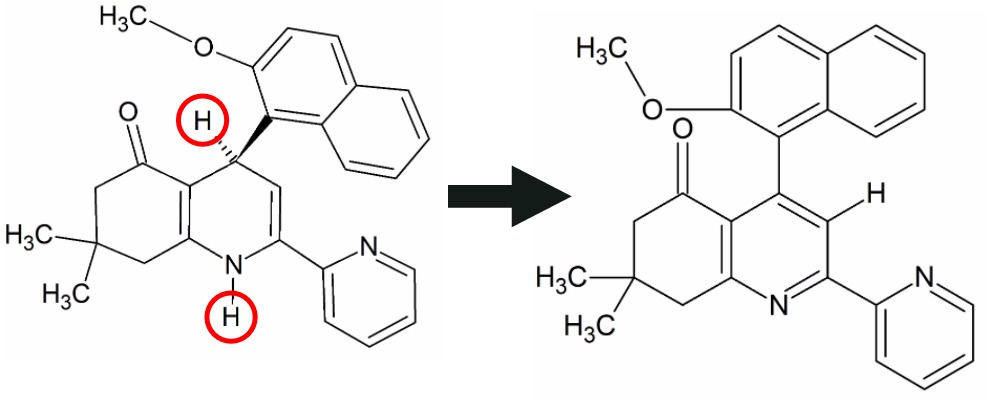
\includegraphics[scale = 0.3]{a}
\end{center}


Comme exposé en introduction, la réaction de conversion de chiralité étudiée dans ce projet est la transformation de dihydropyridine (DHP) en pyridine. \par
\medbreak
Cette réaction est une réaction d’oxydation: on observe l’élimination de deux atomes d’hydrogènes (entourés en rouge), ainsi que la formation d’une nouvelle double liaison.  On remarque également que l’intégralité de la réaction se fait au niveau du cycle principal, sans que le reste de la molécule ne soit modifié.
Afin de réaliser cette réaction, il est donc nécessaire de trouver un réactif dont les affinités avec la DHP lui permettront de retirer ces deux atomes d’hydrogènes. De par les effets inductifs internes au cycle et au besoin de respecter la règle de l’octet, les doubles liaisons du cycle principal se briseront et se reformeront afin de former le cycle aromatique* que l’on observe sur le schéma de la pyridine.
\medbreak
C’est donc cette réaction qui va provoquer la conversion de chiralité. En effet, l’atome d’hydrogène le plus au centre de la molécule de DHP est relié à son centre stéréogène. Après réaction, cet atome de carbone asymétrique n’en est plus un, car n’est plus lié qu’à trois atomes. La molécule de pyridine n’a donc plus de centre stéréogène. 
\medbreak

\begin{center}
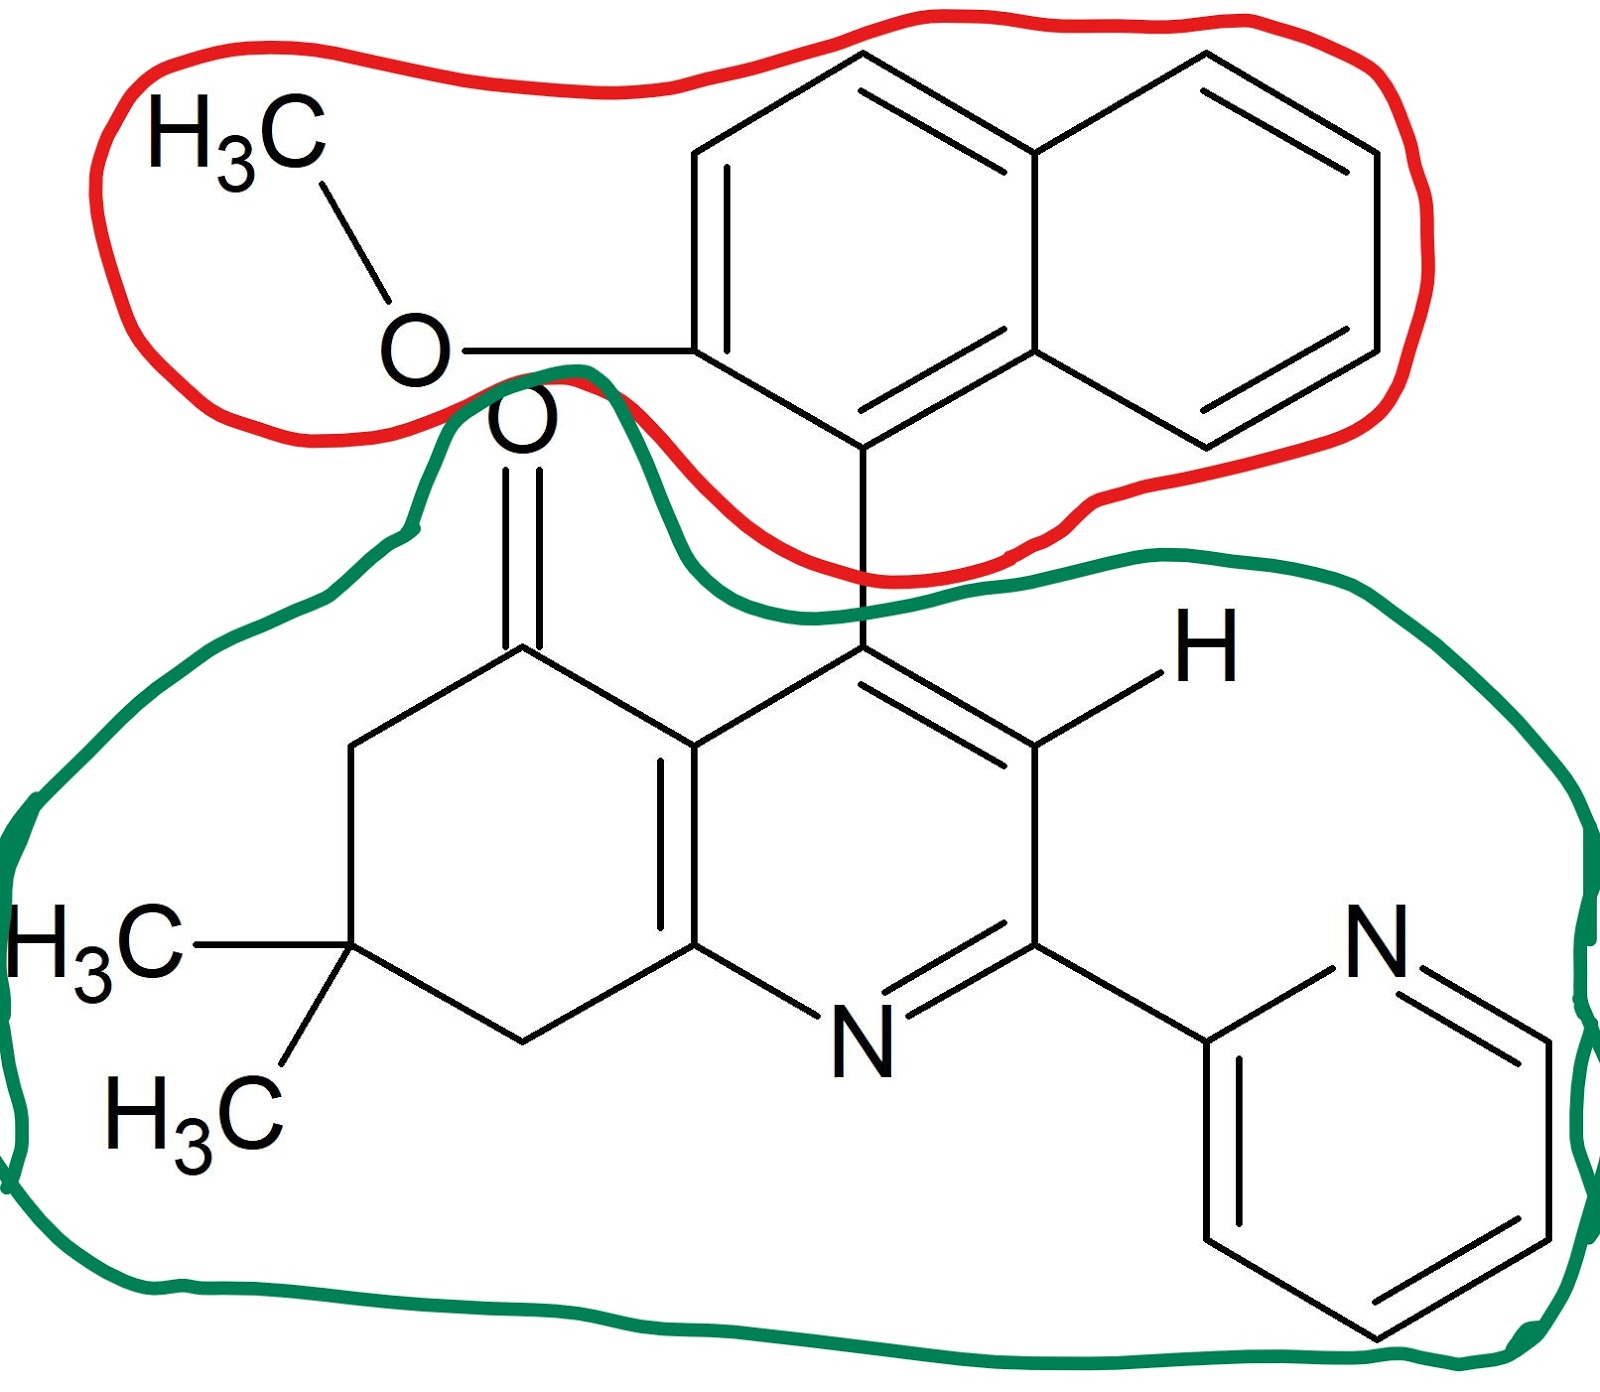
\includegraphics[scale = 0.1]{b}
\end{center}

Cependant, cette molécule possède une nouvelle caractéristique: Lorsque le groupement ici entouré en rouge effectue une rotation autour de l’axe liant les deux groupes colorés, un blocage est observé avec la liaison C=O du groupe vert. La pyridine n’a donc pas une rotation totalement libre. Due à cette propriété, cette molécule est dite à chiralité axiale, car c’est la rotation des deux groupes autour de l’axe central (et non d’un carbone) qui détermine la configuration de la molécule. Elle est également appelée atropoisomère, due au blocage observé. Deux énantiomères différents sont alors observés, nécessitant une certaine énergie pour passer de l’un à l’autre. Si la barrière de l’énantiomérisation ne correspond pas au brisage d’une liaison mais plutôt à une déformation de la liaison à l’origine du blocage, l'énergie qu’elle demande est suffisamment haute pour être considérée comme semblable.
\medbreak
\medbreak
D’un point de vue énergétique, on observe que les deux groupes de la molécule de pyridine sont semblables à deux plans, perpendiculaires l'un à l'autre, ce qui limite les interactions entre les groupes de part et d'autre de l'axe de chiralité, alors que les groupes de la DHP sont plus inclinés l’un sur l’autre. Ceci augmente donc les interactions internes aux atomes de la DHP.
D’autre part, on observe la formation d’un cycle aromatique au niveau du cycle central de la pyridine, qui n’était pas présent sur la dihydropyridine. Comme le reste de la molécule n’est pas modifiée par cette transformation, l’apparition de ce cycle aromatique est bénéfique pour la stabilité de la molécule, après réaction. Autrement dit, la réaction de conversion de chiralité se fera ici majoritairement dans un sens, les molécules de pyridine étant plus stables que celles de dihydropyridine.
\medbreak
Nous avons d'abord essayé d'analyser la nature de la réaction qui permet de passer de dihydropyridine à la pyridine. Il s'agit d'une réaction d'oxydation, qui élimine une molécule de dihydrogène. A travers cette réaction, une des doubles liaisons du cycle principal est brisée et deux autres sont formées.
\medbreak
\subsection{Contrôle de la position des deux sous-groupes}

Nous nous sommes ensuite intéressé à l’importance du contrôle des groupes (vert et rouge) de la DHP. En effet, nous avons rapidement observé que c’est justement cette orientation qui est l’élément crucial de notre réaction énantiosélective, c’est elle qui va définir si la molécule produite sera l’énantiomère (aS) ou (aR) de la pyridine.
\medbreak
Si on ne considère qu’un seul des deux énantiomères de la DHP, on peut en effet obtenir les deux énantiomères de la DHP, sans aucune sélectivité, si on considère que la rotation sur la DHP est libre.
On peut ainsi parler ici de pseudo-diastéréoisomérie, en assumant que la barrière de rotation du groupement est suffisamment élevée pour nécessiter une quantité d'énergie assimilable au brisage d’une liaison. Cette dénomination est cependant relative, car la barrière de rotation dépend des conditions de l’expérience (en particulier, elle varie avec la température).
\medbreak
Il en vient ainsi que l’étude et le contrôle de cette rotation sont capitaux pour notre réaction. Dans la prochaine partie, nous aborderons les concepts de “barrières énergétiques de rotation” dont nous avons parlé précédemment et de chemins réactionnels, qui définissent la réaction globale ainsi que les proportions des énantiomères produits. Ces concepts nous permettent ainsi de quantifier ce que l’on observe qualitativement, et de nous donner des éléments pour choisir un réactif adéquat.
\begin{center}
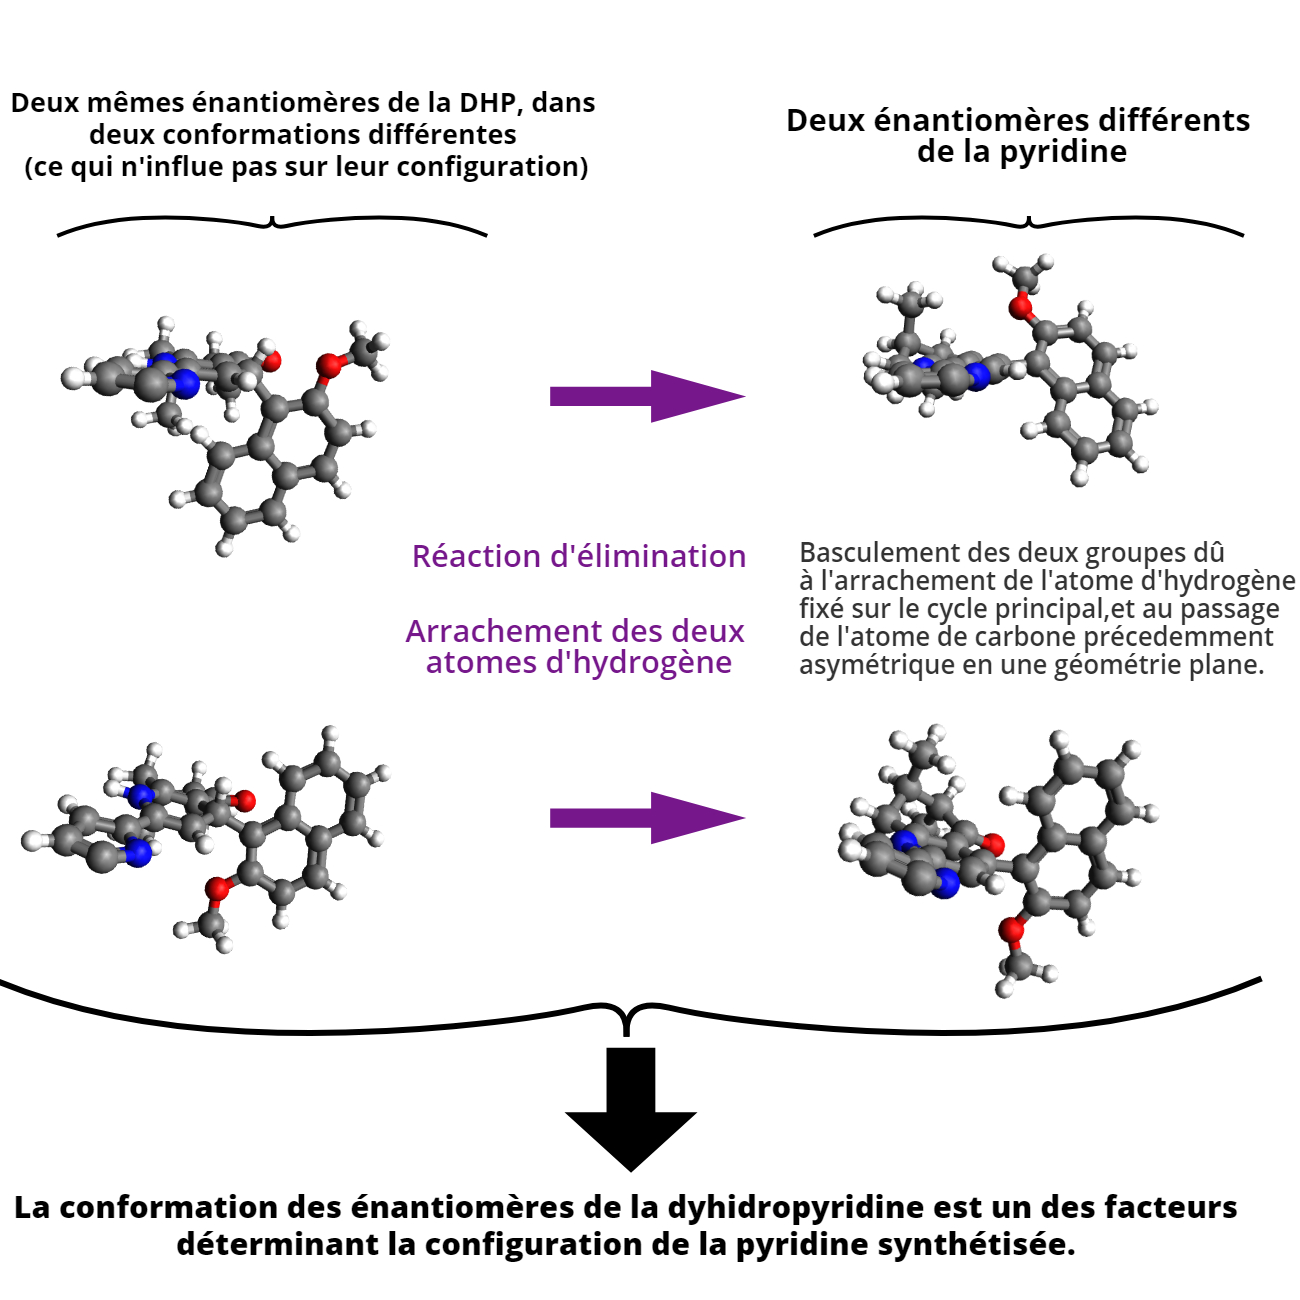
\includegraphics[scale = 0.35]{c}
\end{center}
\newpage
\section{Aspect énergétique et chemins réactionnels}

Il est donc nécessaire de comprendre comment varie cette barrière énergétique qui a été observée dans la première partie. Comme c’est elle qui détermine en grande partie le ratio d’énantiomères produits, il est important de connaître son ordre de grandeur, afin de savoir si cette rotation des groupes est plutôt “libre” (barrière énergétique faible) ou “bloquée” (barrière énergétique haute).

\subsection{Barrière rotation et enthalpie libre d’activation}

\subsubsection{Barrières de rotations}

La barrière de rotation correspond à l'énergie d'activation permettant de passer d'une conformation à une autre autour d'une liaison simple. L’énergie d’activation étant l’énergie à fournir pour qu’une réaction ait lieu.
\medbreak
Cette barrière trouve son origine dans des interactions dues aux forces de Coulomb ainsi qu’au force de van der Waals. Dans le cadre de notre projet, cette grandeur est particulièrement importante car c’est elle qui nous permettra de quantifier la difficulté de passage d’une conformation à une autre pour la molécule. On pourra ainsi mieux comprendre s’il est possible de “bloquer” certaines conformations, ou bien au contraire de passer rapidement de l'une à l'autre. C’est un point primordial dans le cadre de notre synthèse énantiosélective. Comme dit précédemment, c’est justement la conformation de la dihydropyridine qui détermine la configuration de la pyridine que l’on produira. 
\medbreak
On peut, par simulation ou expérimentalement, déterminer les constantes de vitesse k de la réaction de passage d’une conformation à une autre. Ces constantes peuvent être utilisé dans l’équation d’Eyring afin de déterminer la barrière de rotation.
De plus, connaissant les deux constantes de vitesses, l'équilibre K est défini comme le rapport des constantes de vitesse : $K=\frac{k^1}{k^{-1}}$

Finalement, nous savons que ces barrières varient en fonction des critères de l'environnement comme la température, le solvant ou les réactifs. L’intérêt pour nous ici va donc être de jouer sur ces facteurs afin d’avoir des préférences pour certaines réactions à réaliser, toujours dans l’optique d’une énantiosélectivité.
\medbreak

\subsubsection{Notion d'enthalpie libre}

Pour étudier les différences énergétiques entre les molécules, nous devons nous intéresser aux notions d’entropie et d’enthalpie propres aux molécules. Cependant les molécules étudiées sont des isomères. Nous considérerons donc que les différences d’entropie entre les conformations et configurations sont négligeables. Ainsi, nous ne nous intéresserons qu'à la différence d'enthalpie libre des molécules.

L'enthalpie libre est une fonction d'état que l’on nomme également potentiel thermodynamique, donc ici propre à la molécule étudiée. Cette grandeur nous est particulièrement utile. Elle est tout d’abord reliée aux barrières de rotation des molécules. Mais elle peut surtout être reliée à l’énergie d’activation. En effet, la différence d’enthalpie libre entre un l’état initial et l’état de transition, lorsque l’énergie d’activation a été fournie, correspond à cette même énergie d’activation. On appellera alors cette différence l’enthalpie libre d’activation.



\pparagraph{L'équation d’Eyring}


L’équation d’Eyring relie la vitesse d’une réaction chimique avec la température :
$k=\frac{k_BT}{h}\exp{\dfrac{-\DeltaG^{\ddagger}}}{RT}$ avec k la constante de vitesse, R la constante des gaz parfait, T la température, $k_B$ la constante de Boltzmann, $\DeltaG^{\ddagger}$ l’enthalpie libre d’activation et h la constante de Planck. On remarque que cette relation fait intervenir l’énergie d’activation, ici $\DeltaG^{\ddagger}$ . Il va alors être possible de relier cette énergie avec le coefficient de vitesse k. 
\medbreak

En jouant sur cette énergie d'activation, on a remarqué que cela nous permettrait de préférer certaines réactions à d'autres, voire même à en bloquer certaines, si leur énergie d'activation était trop grande.


\medbreak

Il semble donc important de trouver un réactif qui fera en moyenne plus une réaction que l'autre, peut-être en interagissant avec certains atomes d'oxygène. Il semble également logique que retirer les deux hydrogènes nécessaires pour former la pyridine est un opération qui demandera plus ou moins d'énergie en fonction de l'orientation des groupes de la dihydropyridine.

\medbreak

\pparagraph{Postulat de Hammon}
\par
Ce postulat permet d’envisager la position des états de transition sur les chemins réactionnels et de donner une approximation de l’ordre de grandeur de l’énergie d’activation.
Si la réaction est exothermique(ce qui notre cas) l’état de transition sera près des réactifs et l’énergie d’activation faible.
Si la réaction est endothermique l’état de transition sera proche des produits et l’énergie d’activation élevée
\medbreak
\pparagraph{Estimation de la barrière énergétique}

Afin d’avoir une idée qualitative de l’importance de la barrière d'énergie entre les deux configurations de la pyridine (blocage fort ou faible), nous avons décidé d’utiliser les résultats expérimentaux de la thèse ayant déjà fait cette réaction pour déterminer une valeur du temps de demie-vie à 20°, soit plus ou moins la température du milieu dans lequel nous ferons nos expériences.

A partir de la loi d’Eyring et de la valeur de $k_enantiomérisation = … J.mol^{-1}$ obtenu par la précédente expérience, nous avons pu déterminer que le temps de demie-vie à 20° est d’environ 6000 ans. (Voir calcul complet en Annexe). Ainsi, on peut assumer que cette réaction de passage d’une configuration à une autre est extrêmement lent, et on peut considérer cette réaction comme bloquée.

\medbreak
\subsection{Chemins réactionnels}

Nous allons déterminer théoriquement les chemins réactionnels qui permettraient dans un cas idéal de réaliser cette synthèse énantiosélective, et lequel apparaît comme le plus efficace.  En étudiant la plupart des chemins binaires que l'on peut obtenir (en se restreignant à des états énergétiques "élevé" ou "faible"), on a pu déterminer deux chemins intéressants que nous allons développer plus précisément. L’aspect important des deux cas présentés ci-dessous est le fait qu’ils sont effectués sous contrôle cinétique car les produits que sont les énantiomères de la pyridine ont la même enthalpie libre, ainsi afin de les séparer durant la réaction il faut opérer un contrôle cinétique et non thermodynamique.

\medbreak
              
Le premier scénario valable se place dans le cadre d’un dédoublement cinétique, c’est à dire que le produit qui se forme le plus rapidement est majoritaire. Afin de répondre à cela il faut que les réactions d'oxydations des deux conformations de la DHP s'effectuent à des vitesses différentes. Cela se traduit sur le diagramme énergétique par une énergie d’activation d’oxydation $\Delta G^\ddagger_ox$ (énergie pour lancer la réaction d’oxydation) élevée pour une conformation par rapport à la seconde. Ainsi le fait de passer par des états de transitions qui sont des diastéréomères, entre les conformations de la DHP et les énantiomères de la pyridine, nous permet de réaliser cela. En effet, les diastéréoisomères* ont des enthalpies libres différentes entre eux contrairement aux énantiomères qui ont la même enthalpie libre. De plus, dans ce premier chemin une forte barrière de rotation $\Delta G^\ddagger$ est présente entre les deux conformations, ce qui induit un passage difficile de l'une à l'autre ou très lent.
\medbreak

légende: CR: coordonnées de réaction, G enthalpie libre, ET état de transition(très faible durée de vie), R S pseudo-configuration pour le centre stéréogène des réactifs, aR aS configuration absolue pour l’axe stéréogène des produits, delta G enthalpie d’activation, enthalpie des énantiomères aS et aR inférieur car se sont des aromatiques qui sont plus stables
   
\medbreak
  



Le second chemin réactionnel envisageable est similaire au premier du point de vue des énergies d’activation d’oxydation, seul la barrière de rotation diffère. La barrière de rotation des conformations est relativement faible, ce qui implique un passage rapide de l'une à l'autre et un équilibre rapide. Il faut tout de même noter que les énergies d’activation d’oxydations sont supérieur à la barrière de rotation.
\medbreak

Nous avons conclu que le second chemin est plus adéquat à la réalisation d’une synthèse asymétrique. En effet, dans le premier cas présenté la proportion des produits obtenues est dépendante de la concentration initiale de chaque conformères de la DHP, alors que dans le second scénario cette proportion est seulement due aux enthalpies libres d'activation d’oxydation$\Delta G^\ddagger_{ox}$. Les conformères peuvent avoir des enthalpies libres différentes, ce qui entraîne que l'une des conformations est plus stable, mais comme la barrière de rotation est faible et qu'il y a une différence d’énergie d’activation d’oxydation $\Delta G^\ddagger_{ox}$ seul le conformère le plus réactif réagit.
\medbreak

Notre objectif est donc de se placer dans des conditions expérimentales permettant de tendre vers le second chemin présenté ci-dessus.



\newpage


\section{Résultats expérimentaux}



\subsection{Démarche expérimentale}

La thèse sur laquelle se base notre projet a conclu que le réactif le plus efficace pour effectuer cette réaction de conversion de chiralité est le MnO2. Nous avons ainsi décidé de réutiliser ce réactif et de le traiter de plusieurs manières, en amont de la réaction, et d’observer ainsi les impacts de ce traitement sur le rendement final.
Pour ces expériences, nous avons utilisé une solution racémique de DHP que nous n’avons pas préparée.
\medbreak
La première expérience qui a été réalisé est une expérience témoin avec le Mn02 dans le cyclohexane, et servira d’élément de comparaison pour les trois autres expériences. Cette expérience est réalisée dans les mêmes conditions que celles dans lesquelles a été faite la précédente expérience. ( milieu basique )
 \medbreak
La seconde expérience consiste en l’utilisation de MnO2 sur charbon actif. Nous pensons en effet que le charbon actif, souvent utilisé comme catalyseur, aura un impact de par ses affinités sur la cinétique et l'énantiosélectivité de la réaction. ( milieu basique )
\medbreak
La troisième expérience nous avons utilisé de l’acide trichloracétique dans de l’acétonitrile. ( milieu acide )
Et dans notre dernière expérience nous avons également utilisé de l’acide trichloroacétique mais cette fois mélangé avec du chlorophorme. (milieu acide )
\medbreak
Nous avons laissé les réactions se faire pendant 24h puis nous avons isolé la pyridine.
Une fois isolé nous avons envoyé nos quatre produits aux laboratoire afin qu’il nous fournisse un spectre U.V pour que l’on puisse analyser nos résultats.



\subsection{Analyse des résultats}


























Nos attentes :

























\newpage



\section{Annexe}

\subsection{Définitions}
\medbreak
Chiralité axiale :  

La chiralité axiale est une forme de chiralité caractérisée par un axe stéréogène, au lieu d’un centre stéréogène qui défini la chiralité “habituelle”. Dans ce cas, les deux substituants de part et d’autre de l’axe stéréogène sont dans une disposition spatiale fixée non superposable à son image dans un miroir.    
\medbreak

Enantiomère : 

Deux stéréo-isomères de molécules chirales sont dites énantiomères l’une de l’autre si elles sont images l’une de l’autre dans un miroir, mais ne sont pas superposables. C’est le cas ici des deux configurations de la molécule de dihydropyridine, et également de la pyridine.

\medbreak
Diastéréoisomère : 

Deux stéréo-isomères de molécules chirales sont dites diastéréoisomères l’une de l’autre si elles ne sont pas image l’une de l’autre dans un miroir. 
\medbreak
Racémique :

Un racémique est un mélange de deux enantiomère d’une molécule chirale, en proportion égales (50% de l’une, 50% de l’autre). C’est en général ce type de mélange que l’on obtient en synthétisant une molécule chirale sans chercher à contrôler sa chiralité (le plus souvent, dans un milieu non-chiral).

\medbreak
Cycle aromatique: 

Un cycle aromatique est un cycle de carbones comprenant 4n + 2 électrons. L’exemple le plus courant est le benzène. Une des principales caractéristiques du cycle aromatique est la grande stabilité qu’il procure à la molécule dont il fait partie. 

\medbreak
Abréviation: 

DHP = Dihydropiridine




\medbreak

\subsection{Protocoles}

Lors de la première expérience nous avons mélangé 24mg de DHP avec 3,5 mL de cyclohexane et 102 mg de MnO2. Le cyclohexane nous sert ici, ainsi que dans la seconde expérience de solvant.
Pour la seconde expérience nous avons mélangé 24mg de DHP avec 3,5mL de cyclohexane et 102 mg de MnO2 sur charbon actif. 
Dans notre troisième expérience nous avons mélangé 41 mg de DHP avec de l’acide trichloroacétique dans de l’acétonitrile.
Et dans notre dernière expérience nous avons mélangé 41 mg de DHP avec de l’acide trichloroacétique dans du chloroforme.
\medbreak

Une fois ces réactions terminé, il a fallu ensuite isoler la pyridine pour chaque solution. 
\medbreak
Pour les 4 expériences nous avons réalisé une filtration sous vide avec de la célite, car  des impureté se sont formées. Nous avons rajouté du dichlorométhane comme solvant car il ne  réagit pas avec la pyridine, possède une faible température d’ébullition [ je ne me souviens plus du troisième avantage et on ne l’a pas marqué?] …
\medbreak
Nous avons ensuite utilisé deux méthodes différentes pour isoler notre produit selon les réactifs utilisés.
Pour nos deux réactions en milieux basique nous avons fait une distillation car le dichlorométhane a réagi  avec le Mn02 et possède comme vu précédemment une faible température d’ébullition.
Pour les deux réactions en milieux acide nous avons effectué une extraction en ajoutant du carbonate de sodium ( une base ) afin qu’elle réagisse avec l’acide et forme la phase aqueuse  moins dense que la phase organique. De cette façon nous avons pu récupérer notre phase organique contenant notre produit, nous avons répété cette opération trois fois pour plus de précision. Pour retirer totalement l’eau présente dans notre solution on avons ajouté du sulfate de magnésium anhydre MgSO4. Ce dernier va précipiter en présence de l’eau. Une simple filtration a suffi pour l’enlever de la solution.  Enfin nous avons terminé par une distillation pour enlever le dichlorométhane encore présent de la première filtration.
Enfin pour nos 4 solutions on fait un chromatographie sur colonne avec de la Silice pour enlever les dernières impuretés, et  pour bien vérifier la pureté de nos produit nous avons réalisé une chromatographie sur couche mince avec un produit témoin.




\medbreak

\subsection{Calculs}

\subsubsection*{Calcul du temps de demie-vie de la pyridine}

\end{document}
